\bluepage{OpenGL}

\begin{frame}
\frametitle{OpenGL}
  \begin{itemize}
  \item OpenGL Open Graphics Language (Library) 
  \item OpenGL je API pro 3D grafiku 
  \item Vychází z IrisGL od SGI 
  \item Platformně nezávislé 
  \item Použitelné skoro z každého jazyka 
  \item Slouží pro převod scény popsané primitivy (body, čáry trojúhelníky)  na 2D rastr obrazovky.
  \item V novější verzi (4.3) i pro GPGPU
  \item Obsahuje vlastní jazyk GLSL pro programování GPU
  \end{itemize}
  \begin{figure}[h]
  \includegraphics[width=5cm,keepaspectratio]{pics/opengl/logo}
  \end{figure}
\end{frame}

\begin{frame}
\frametitle{OpenGL - proč používat?}
  \begin{itemize}
    \item{OpenGL je multiplatformní - Linux, Window, Mac Os X, Android,...}
    \item{OpenGL lze použít téměř z každého jazyka - C, C++, Python, Java, Javascript, ...}
    \item{OpenGL je zpětně kompatibilní}
    \item{OpenGL je nízkoúrovňové}
    \item{OpenGL má jednoduché API}
    \item{OpenGL je rychlé}
    \item{OpenGL je otevřený industriální standard}
    \item{WebGL}
  \end{itemize}
\end{frame}


\begin{frame}
\frametitle{Verze OpenGL}
  \begin{itemize}

  \item{OpenGL}
  \begin{itemize}
  \item{1.x - fixní pipeline}
  \item{\textbf{2.x} - programovatelná pipeline}
  \item{3.x - geometry shader, \textbf{Deprecation}}
  \item{4.x - Hardwarová tesselace, dvojitá přesnost}
  \item{4.3 - Compute shadery}
  \item{4.5 - Direct State Access}
  \end{itemize}

  \item{OpenGL ES}
  \begin{itemize}
  \item{Vestavěné systémy, mobily, tablety}
  \item{1.x - fixní pipeline}
  \item{\textbf{2.x} - programovatelná pipeline}
  \item{3.x - Occlusion queries, 3D textury, transform feedback}
  \end{itemize}

  \item{WebGL}
  \begin{itemize}
  \item{OpenGL ve webovém prohlížeči}
  \item{\textbf{Velmi podobné OpenGL ES}}
  \end{itemize}

  \end{itemize}
\end{frame}

\begin{frame}
\frametitle{OpenGL}
  \begin{itemize}
    \item{OpenGL je architektura klient server}
    \item{Aplikace běží na CPU a využívá OpenGL pro přístup k GPU}
  \end{itemize}
  \begin{figure}[h]
    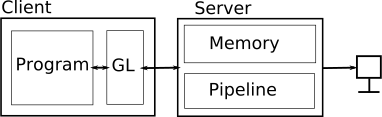
\includegraphics[width=10cm,keepaspectratio]{pics/opengl/clientserver}
  \end{figure}
\end{frame}

\begin{frame}
\frametitle{OpenGL}
	\begin{picture}(320,250)
		\put(-25,70){\includegraphics[width=12.5cm,keepaspectratio]{pics/opengl/RenderingPipeline}}
	\end{picture}
\end{frame}

\begin{frame}
\frametitle{OpenGL API}
  \begin{itemize}
    \item Jednoduché rozhraní
      \begin{itemize}
        \item Pouze C funkce
        \item Data jsou jen čísla a pole
        \item Žádné struct, class
      \end{itemize}
    \item Stavový stroj
      \begin{itemize}
        \item Většina příkazů nastavuje stav pipeline
        \item Stav se sám nemění
      \end{itemize}
    \item OpenGL (Rendering) Context
      \begin{itemize}
        \item Hlavní objekt OGL
        \item Mimo OpenGL (WGL/GLX)
        \item Zapouzdřuje data, stav, napojení na výstup
      \end{itemize}
  \end{itemize}
\end{frame}

\begin{frame}
\frametitle{Příkazy a typy}
  glName{\it NT}(...)
  \begin{itemize}
    \item N - počet parametrů
    \item T - typ parametrů
  \end{itemize}
    \begin{tabular}{|l|l|l|l|}
    \hline
    b & 8b integer & signed char & GLbyte \\ \hline
    s & 16b integer & short & GLshort \\ \hline
    i & 32b integer & long & GLint,GLsizei \\ \hline
    f & 32b float & float & GLfloat,GLclampf \\ \hline
    d & 64b float & double & GLdouble,GLclampd \\ \hline
    ub & 8b unsigned & unsigned char & GLubyte,GLboolean \\ \hline
    us & 16b unsigned & unsigned short & GLushort \\ \hline
    ui & 32b unsigned & unsigned long & GLuint,GLenum,GLbitfield \\ \hline
    *v & Ukazatel a * & & \\ \hline
    \end{tabular}
    GLvoid glUniform2f(GLuint,GLfloat,GLfloat);
    GLvoid glUniform2fv(GLuint,GLfloat*);
\end{frame}

\begin{frame}
\frametitle{Příkazy a typy}
  OpenGL příkazy lze rozdělit do několika skupin
  \begin{itemize}
    \item \textbf{Příkazy pro správu OpenGL objektů (10 hlavních OpenGL objektů)}
    \item \textbf{Exekuční příkazy (kreslící a výpočetní příkazy)}
    \item \textbf{Stavové příkazy (nastavují globální stav OpenGL, příkazy pro zjištění stavu)}
    \item Debugovací příkazy
    \item Operace s framebufferem
    \item Příkazy pro synchronizaci (glFinish)
    \item Utilitní příkazy
  \end{itemize}
\end{frame}


\begin{frame}
\frametitle{OpenGL Objekty}
  GLvoid glGen{\it Objects}(GLsizei n,GLuint * objects);\\
  GLvoid glDelete{\it Objects}(GLsizei n,const GLuint * objects);
  \begin{itemize}
    \item Jméno objektu - GLuint, všechny objekty jsou v API reprezentovány integerem
    \item 0 rezervována pro prázdný objekt
  \end{itemize}
  Objekty:
  \begin{itemize}
    \item \textbf{Program}
    \item \textbf{Shader}
    \item \textbf{Buffer}
    \item \textbf{Vertex Array Object}
    \item Texture
    \item Framebuffer
    \item Renderbuffer
    \item Sampler
    \item Asynchronous Query
    \item ProgramPipeline
  \end{itemize}
\end{frame}

\begin{frame}
\frametitle{Způsob využití OpenGL pro kreslení}
  \begin{itemize}
    \item Pro vykreslení grafiky pomocí OpenGL je potřeba inicializovat několik objektů
    \item Shader Program(y), Buffer(y), Vertex Array Object(y)
    \item Inicializace spočívá v kompilaci a likování programů
    \item Alokaci a kopírování dat na GPU
    \item Konfigurace stavů OpenGL a konfigurace čtení z GPU paměti
    \item Spuštění kreslení pomocí vykreslovacích příkazů
  \end{itemize}
\end{frame}


